\chapter{Introduction}

A Distributed Computing System is a concept where a network of multiple nodes works on a single problem. In Distributed Computing a problem is divided into smaller parts and solved by different notes. The nodes can be physically close, connected via a local network, or geographically distant, connected by a wide area network. The goal of a distributed computing is to make such a node network act as a single computer.

\begin{figure}
	\centering
	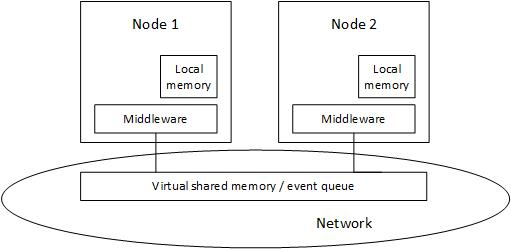
\includegraphics[width=0.8\textwidth,natwidth=610,natheight=642]{DistributedComputingSystemWith2nodes.jpg} 
	\captionsetup{format=plain,font=footnotesize,labelfont={bf,red},labelsep=quad,singlelinecheck=no}
	\caption[Distributed Computing System with 2 nodes]{
		\label{fig:distributedCoputingSystem} 
		\footnotesize{%
			A Distributed Computing System with 2 nodes.
		}
	}
\end{figure}

Figure \cref{fig:distributedCoputingSystem} illustrates the idea of a distributed computing system. Nodes 1 and 2 shares some virtual memory and/or event queue. The Middleware is a handles communication between the nodes and ensures the virtual memory is consistent throughout the network. The shared virtual memory is transparent to each node. 

Distributed systems offer many benefits over centralized systems including the following:
\begin{itemize}
	\item Scalability: It is easy to add notes to the system, should the size of the system increase.
	\item Redundancy: Several nodes can provide the same service, so if a node crashes, there are many to replace it. Additionally, from a cost perspective, each node does not have to be expensive, because many smaller nodes can be used as replacement.
\end{itemize}

\section{Thesis motivation}

\subsection{Siemens case}
Siemens Wind Power is among the leading windmill manufacturers in the world. 
Siemens builds wind farms of different sizes ranging form single mills to well above one hundred windmills \cite{simensOffShoreProjects, simensOnShoreProjects}.

In the current setup (see \cref{fig:currentSiemensSetup}) the Park Monitor is a central component and a SPOF (single point of failure).
The system is running on windows with a MSSQL database in the Park Monitor and MySQL on the windmills them self.
The windmills, Park Monitor and Park Regulator is connected with a gigabit network, witch currently has plenty of extra capacity.
The system handles more than 50 control points and 200 measurement points, and samples these every 50 ms.
The Park regulator is associated with the transformer station and regulated the power production when needed.
This component currently has a less than optimal work flow see \cref{fig:dataComputationSequence}.

Siemens has a need for their system to scale better and provide increased redundancy to avoid these SPOF's.
Siemens has a vision of removing the Park Monitor component and make it into a distributed system, distributed among the windmills (see \cref{fig:futureSiemensSetup}).
Also Siemens would like to look for ways to optimise the calculations done by the Park Regulator, 

\begin{figure}
	\centering
	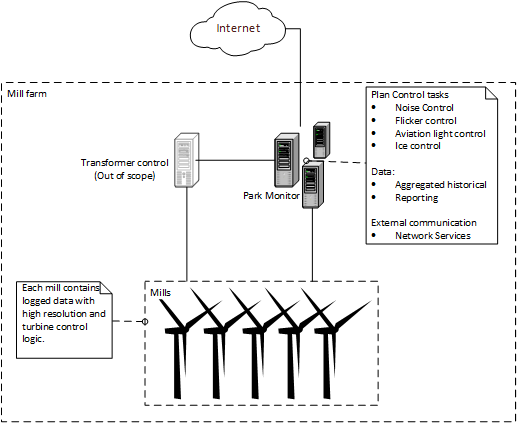
\includegraphics[width=0.7\textwidth,natwidth=610,natheight=642]{SystemOverviews.png} 
	\captionsetup{format=plain,font=footnotesize,labelfont={bf,red},labelsep=quad,singlelinecheck=no}
	\caption[Illustrates the current Siemens windmill farm setup]{
		\label{fig:currentSiemensSetup} 
		\footnotesize{%
			This figure illustrates the current Siemens windmill farm setup.
		}
	}
\end{figure}

\begin{figure}
	\centering
	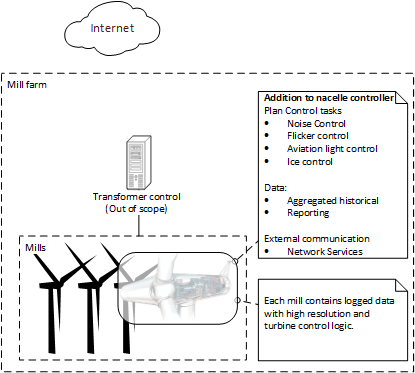
\includegraphics[width=0.7\textwidth,natwidth=610,natheight=642]{SystemOverviewsFuture.png} 
	\captionsetup{format=plain,font=footnotesize,labelfont={bf,red},labelsep=quad,singlelinecheck=no}
	\caption[Illustrates the future Siemens windmill farm setup]{
		\label{fig:futureSiemensSetup} 
		\footnotesize{%
			This figure illustrates the future Siemens windmill farm setup.
		}
	}
\end{figure}

\begin{figure}
	\centering
	\begin{sequencediagram} %Created using pgf-umlsd
		\newthread{reg}{:Park Regulartor}
		\newinst[2]{mill}{:Mill}
	
		\begin{sdblock}{each mill}{}
			\mess[1]{reg}{getCurrentStatus}{mill}
			\mess[1]{mill}{status}{reg}	
		\end{sdblock}
		
		\begin{call}{reg}{calculateAllSetpoints()}{reg}{}
		\end{call}
	
		\begin{sdblock}{each mill}{}
			\mess[1]{reg}{setNewSetpoint}{mill}
		\end{sdblock}
					
	\end{sequencediagram}

	\captionsetup{format=plain,font=footnotesize,labelfont={bf,red},labelsep=quad,singlelinecheck=no}
	\caption[Regulator calculation sequence]{
		\label{fig:dataComputationSequence} 
		\footnotesize{%
			Regulator calculation sequence.
		}
	}
\end{figure}
















\subsection{et eller andet}

Today windmills in windmill farm at Siemens are equipped with a computer for regulation, data and communication purposes. Every windmill are connected to a single server that aggregates data, perform calculations, store data and handle communication with the outside world. At Siemens up to 8 of theses servers are present pr. windmill farm and they pose the following problems:
\begin{itemize} 
	\item Single point of failure. Should a server fail, a part of the windmill farm will become unavailable.
	\item Low scalability. The servers does not scale with the number of windmills.
	\item Up performance of park regulator.
\end{itemize}

Therefor Siemens wishes to remove the servers by making every windmill farm a Distributed Computing System, utilizing free capacity of the computers already residing in every windmill. This would up the redundancy and scalability and the remove possibility of a single point of failure. A windmill farm must serve as single server which means ease of access must be maintained even though computation and data is distributed. This means routing traffic to a windmill with free capacity through a single interface, without external systems being aware of it.

% Today windmills in windmill farm are connected to a single server that aggregates data, perform calculations, store data and handle communication with the outside world. These servers do not scale well with the size of the windmill farm, and they are a single point of failure. Therefor Siemens wishes to remove the servers by utilizing free capacity of the computers already residing in every windmill. 
%Currently there is some limited redundancy in data and availability but this could be greatly improved by distributing data and communication to the windmills. 
%Ease of access must be maintained even though computation and data is distributed. 
%This means routing traffic to a windmill with free capacity through  a single interface.

\section{Thesis aim}

The purpose of this thesis is to design, implement and evaluate a framework and associated tools for distributed computing systems development. The case from Siemens Windpower is an example of a production environment where the framework could be utilized. The goal is not to make a framework that is specific to the Siemens case but to make a general framework for this and similar cases. 

This framework must be able to handle computation distributed on several nodes, communication between those nodes and distribution of data. 

The framework will be evaluated with regards to the existing Siemens solution using the following parameters: ... and will be done by comparing results obtained from a protocol 


%\begin{itemize}
%	\item How do we distribute a database and computation across a production environment in the best possible way?
%	\item How do we define and measure performance?
%	\item Can it provide data redundancy and outperform current systems?
%	\item How many windmills are needed before it makes sense to makes sense to distribute the server?
%\end{itemize}
%
%We aim to investigate the possibility of making a framework and associated tools for developing a distributed system. 
%This framework must be able to handle computation distributed on several nodes, communication between those nodes and distribution of data. 
%The communication can be built on top of existing standards as for instance DDS. Data distribution can be built using existing systems like MongoDB. 
%Distribution of computation tasks is the main research area and will be the focus of this thesis.
%
%In order to achieve distributed computation on several nodes the framework must be able to perform load balancing and control the distribution of tasks on the nodes in the system. 
%Furthermore the framework must have a single interface for control of, and interaction with, all the nodes.  
%The goal is to create a test system, that can distribute and perform tasks but also to be able to plan ahead of time and know if there is available computation time.
%
%The case from Siemens Windpower is an example of a production environment where the framework could be utilized. 
%Our goal is not to make a framework that is only  specific for this case but to make a general framework for this and similar cases.

\section{Approach}

\section{Outline}
The remainder of this thesis is organized into the following chapters...

\section{Audience}
This thesis is aimed at an audience with a basic knowledge of...
